%%%%%%%%%%%%%%%%%%%% author.tex %%%%%%%%%%%%%%%%%%%%%%%%%%%%%%%%%%%
%
% sample root file for your "contribution" to a proceedings volume
%
% Use this file as a template for your own input.
%
%%%%%%%%%%%%%%%% Springer %%%%%%%%%%%%%%%%%%%%%%%%%%%%%%%%%%


\documentclass{svproc}
%
% RECOMMENDED %%%%%%%%%%%%%%%%%%%%%%%%%%%%%%%%%%%%%%%%%%%%%%%%%%%
%

% to typeset URLs, URIs, and DOIs
\usepackage{url}
\usepackage{amsmath}
\usepackage{algorithm}
\usepackage[noend]{algpseudocode}

\usepackage{graphicx}

%\usepackage{caption}
%\usepackage{subcaption}
%\captionsetup{compatibility=false}

% Springer does not support subcaption/caption => use subfig instead and avoid loading the caption package
\usepackage[caption=false]{subfig}

\usepackage{siunitx}
\usepackage{amsmath}
\usepackage{tikz}
\usepackage{adjustbox}

\usepackage{ upgreek }

\usetikzlibrary{arrows, arrows.meta, fit, positioning, quotes,
                shadows, shapes.geometric, shapes.misc}





\def\UrlFont{\rmfamily}

%%%%%%%%%%%%% math stuff
\usepackage{amssymb}

%flowchart definitions
\tikzstyle{startstop} = [rectangle, rounded corners, minimum width=3cm, minimum height=1cm,text centered, draw=black, fill=red!30]
\tikzstyle{io} = [trapezium, trapezium left angle=70, trapezium right angle=110, minimum width=3cm, minimum height=1cm, text centered, draw=black, fill=blue!30]
\tikzstyle{process} = [rectangle, minimum width=1cm, minimum height=1cm, text centered, draw=black, fill=white!30]
\tikzstyle{decision} = [diamond, minimum width=1cm, minimum height=1cm, text centered, draw=black, fill=cyan!30]
\tikzstyle{arrow} = [thick,->,>=stealth]

\tikzset{
  font={\fontsize{11pt}{12}\selectfont}}


% vectors in bold
\newcommand{\vp}{\mathbf{p}}
\newcommand{\valpha}{\mathbf{\alpha}}
\newcommand{\vP}{\mathbf{P}}
\newcommand{\vg}{\mathbf{g}}
\newcommand{\vf}{\mathbf{f}}
\newcommand{\vw}{\mathbf{w}}
\newcommand{\vx}{\mathbf{x}}
\newcommand{\vq}{\mathbf{q}}
\newcommand{\vzero}{\mathbf{0}}
\newcommand{\vn}{\mathbf{n}}
\newcommand{\vo}{\mathbf{o}}
\newcommand{\vchi}{\mathbf{\chi}}
\newcommand{\vlbA}{\mathbf{lbA}}
\newcommand{\vubA}{\mathbf{ubA}}
\newcommand{\vlb}{\mathbf{lb}}
\newcommand{\vub}{\mathbf{ub}}


% sets as caligraphics
\newcommand{\cV}{\mathcal{V}}
\newcommand{\cS}{\mathcal{S}}
\newcommand{\cC}{\mathcal{C}}
\newcommand{\cE}{\mathcal{E}}
\newcommand{\cO}{\mathcal{O}}

% misc
\newcommand{\R}{\mathbb{R}} % real numbers

%%%%%%%%%%%%%
\newcommand{\todo}[1]{\textbf{\textcolor{red}{TODO: #1}}}

\begin{document}
\mainmatter              % start of a contribution
%
% Robust Motion Execution
% 
\title{Distributed Realtime Trajectory Replanning for Robust Motion Execution in Multi-Robot Systems}


%
\titlerunning{Distributed Realtime Trajectory Replanning}  % abbreviated title (for running head)
%                                     also used for the TOC unless
%                                     \toctitle is used
%
\author{Baskin Senbaslar \and Wolfgang H\"onig \and
Nora Ayanian}
%
%\authorrunning{Ivar Ekeland et al.} % abbreviated author list (for running head)
%
%%%% list of authors for the TOC (use if author list has to be modified)
\tocauthor{Baskin Senbaslar, Wolfgang H\"onig, Nora Ayanian}
%
\institute{University of Southern California, Los Angeles CA, USA,\\
\email{\{baskin.senbaslar, whoenig, ayanian\}@usc.edu}}

\maketitle              % typeset the title of the contribution

\begin{abstract}
\keywords{trajectory planning, collision avoidance, multi-robot systems}
\end{abstract}


\section{Introduction}
Motion planning for multi-robot systems is widely used and in particular important in cases where many robots have to interact with each other in confined spaces, potentially with many obstacles around.
Examples include coordination of robots in warehouses~\cite{Kiva}, traffic management at intersections~\cite{IntersectionManagementDresner}, and airport management~\cite{AirportTug}.
Modern planning algorithms can find trajectories that effectively coordinate hundreds of robots while approximately optimizing objectives like total energy used~\cite{crazyplanning-ieeetro}.
However, all such solutions assume that the resulting trajectories can be executed approximately perfectly, which is in particular not true for teams of hundreds of robots that have to operate persistently.

We propose robust motion execution as a framework that take pre-planned trajectories as input and compensate for a variety of dynamic changes, including imperfect motion execution of some robots, newly appearing obstacles, or robots breaking down.
Consider the example in Fig.~\ref{fig:swap2:initial}, where two robots are tasked with swapping their position.
The pre-planned trajectories are collision-free, but neither consider a new obstacle nor that the blue robot does not start it the right location.
Robust motion execution can be used to still successfully swap positions, while staying as close as possible to to the pre-planned trajectories (see Fig.~\ref{fig:swap2:final}).
Our framework is fully distributed and requires no communication; the robots only need to know their own trajectories and need to be able to sense their neighbors' positions and obstacles around them.

\begin{figure}
\centering
\subfloat[Initial configuration.]{
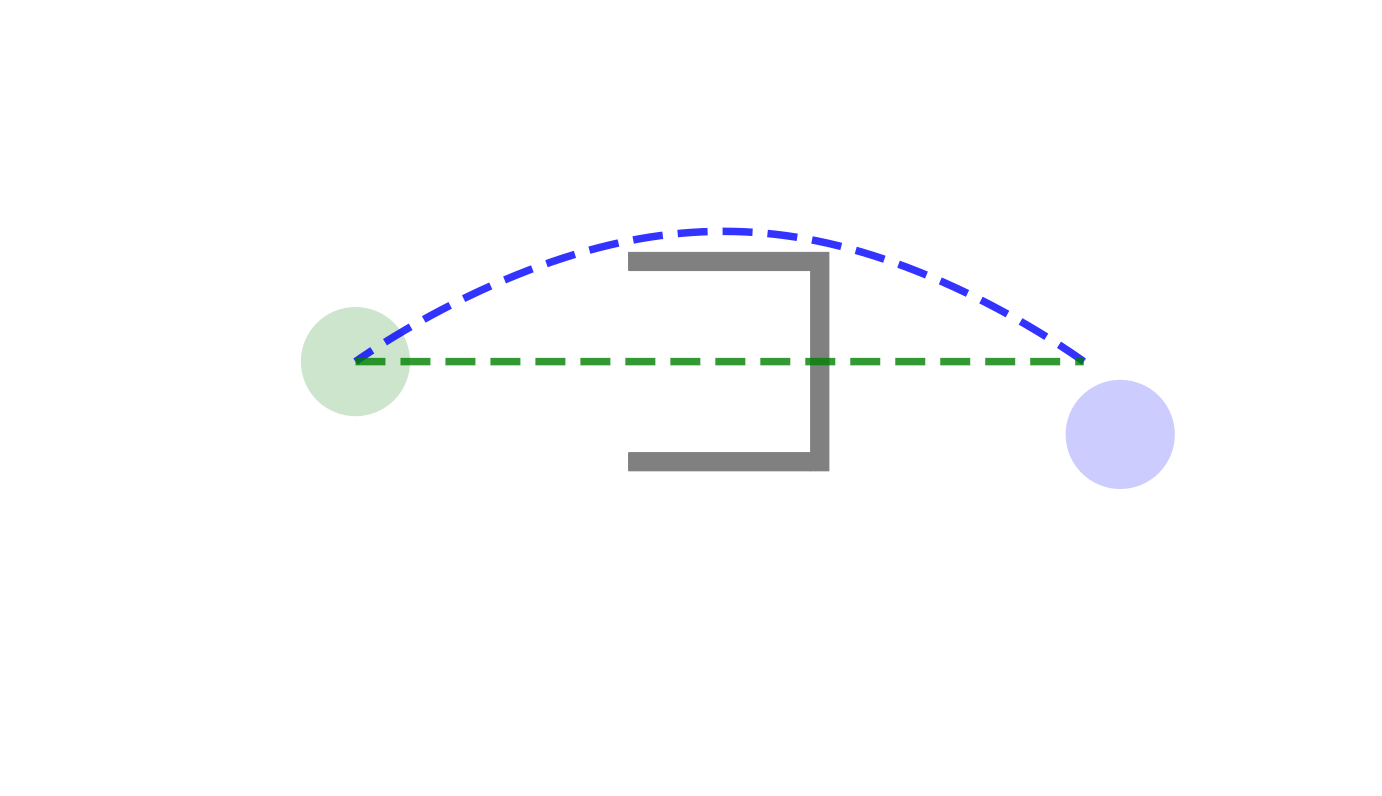
\includegraphics[width=0.48\textwidth]{images/swap2_initial.pdf}
\label{fig:swap2:initial}
}
\hfill
\subfloat[Final configuration and executed trajectories.]{
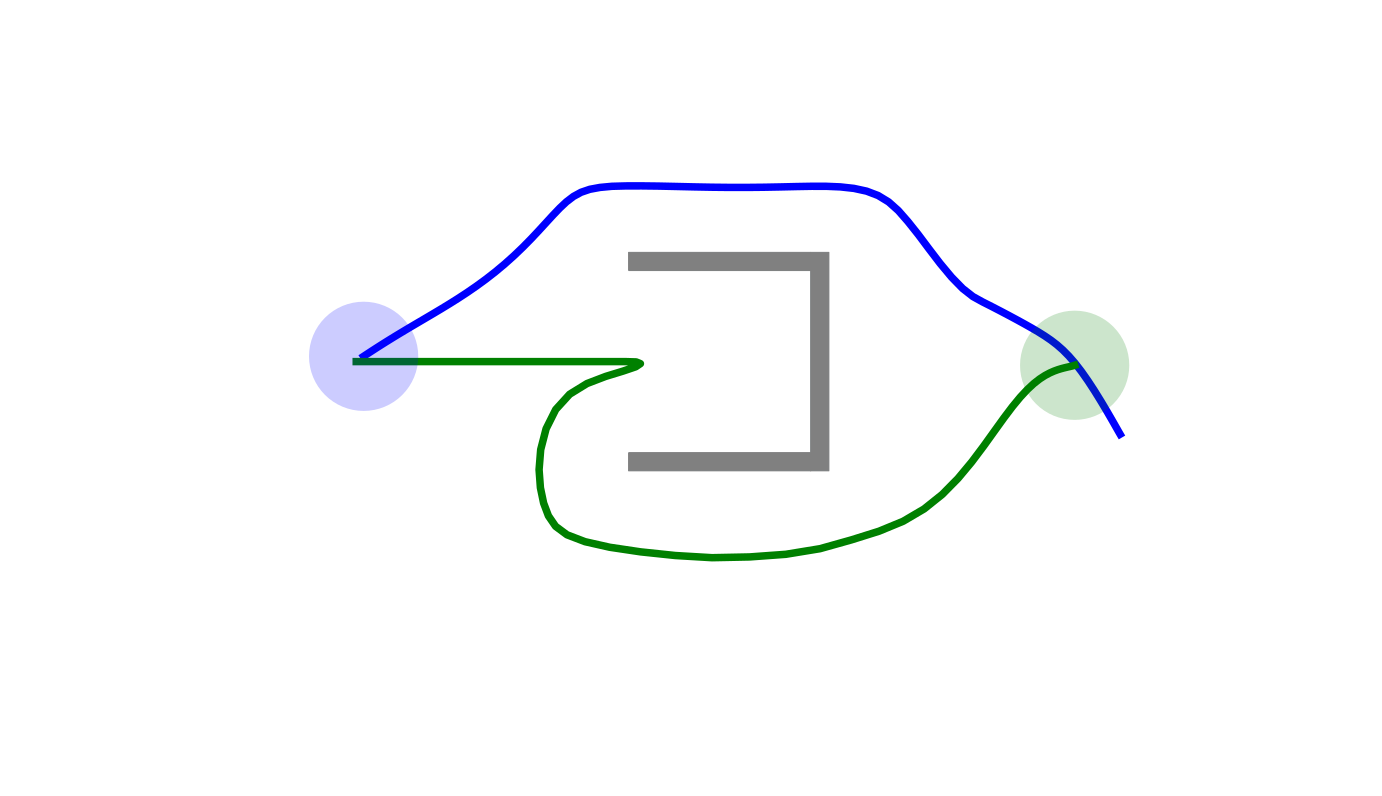
\includegraphics[width=0.48\textwidth]{images/swap2_final.pdf}
\label{fig:swap2:final}
}
%\begin{subfigure}[t]{0.48\textwidth}
%\centering
%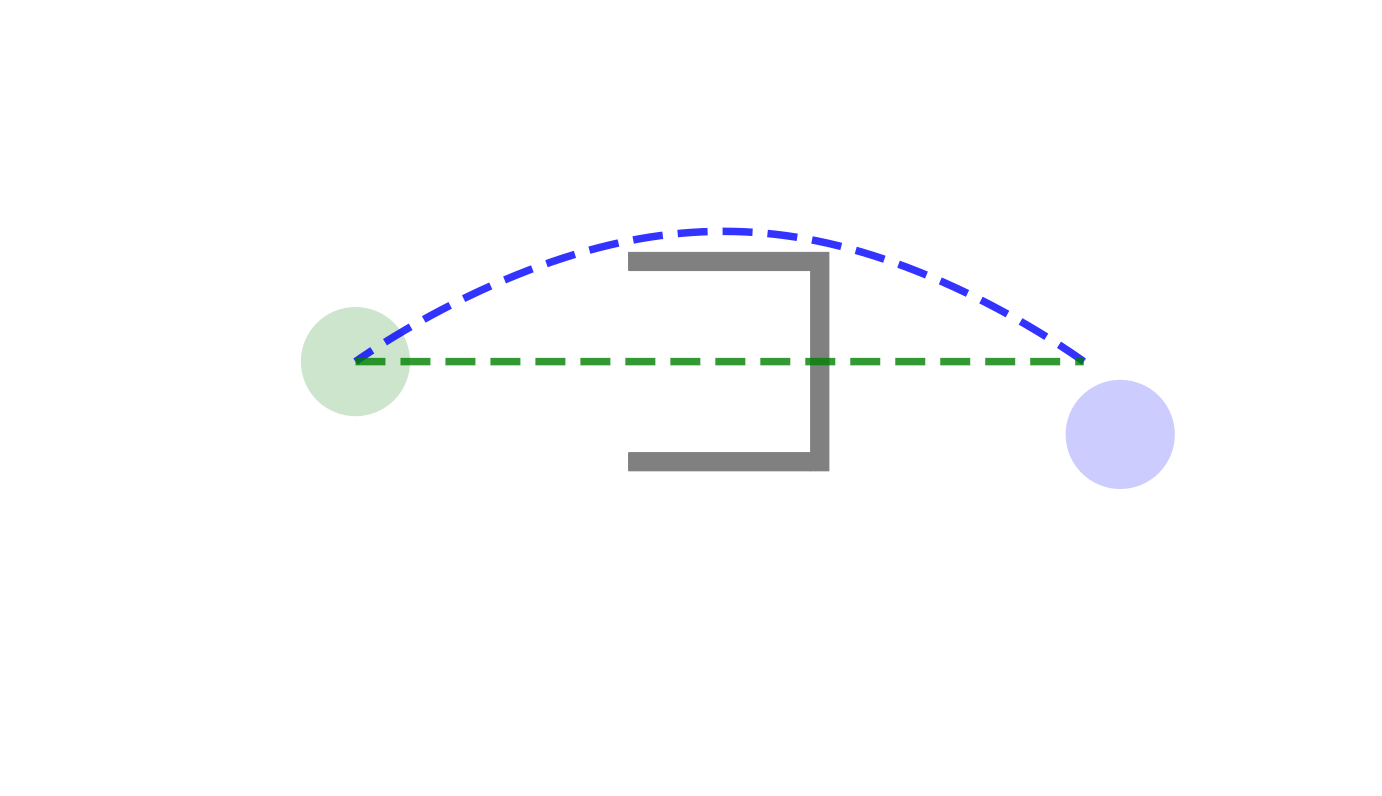
\includegraphics[width=1.0\textwidth]{images/swap2_initial.pdf}
%\caption{Initial configuration.}
%\label{fig:swap2:initial}
%\end{subfigure} \hfill
%\begin{subfigure}[t]{0.48\textwidth}
%\centering
%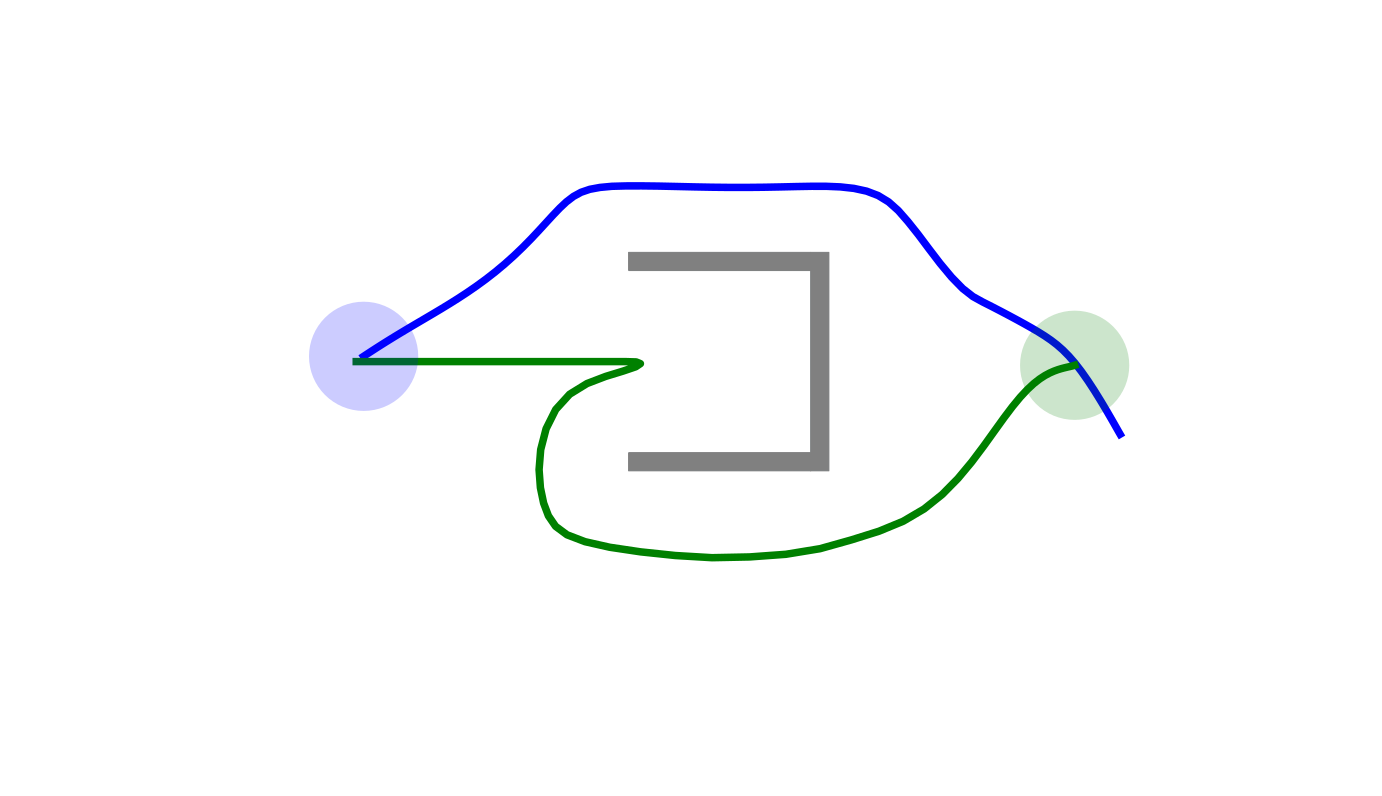
\includegraphics[width=1.0\textwidth]{images/swap2_final.pdf}
%\caption{Final configuration and executed trajectories.}
%\label{fig:swap2:final}
%\end{subfigure}
\caption{Two robots (green and blue circles) are tasked with following their preplanned trajectories (green and blue dashed lines).
The initial plans were created without knowledge of the obstacle (gray) and the blue robot does not start at its planned start position.
Our approach computes smooth trajectories in real-time, avoiding the new obstacle and other robots while staying close to the preplanned trajectory.
}
\label{fig:swap2}
\end{figure}

Robust motion execution is an extension of cooperative collision avoidance where our objective is to stay close to the originally planned trajectories as much as possible.
In contrast, traditional collision avoidance methods frequently only take a desired velocity, desired goal state, or desired action as input (see Section~\ref{sec:relatedWork}).
Our method is based on \emph{Buffered Voronoi Cells} (BVC)~\cite{bufferedVoronoiCells} as the underlying cooperative collision avoidance strategy and retains the same theoretical guarantees.
At the high-level we employ a novel combination of trajectory optimization and discrete search-based planning with dynamic receding horizon.
The discrete search allows us to avoid local minima effectively even in difficult scenarios, while the trajectory optimization takes the dynamics of real physical robots into account.



\todo{perhaps write some more about what experiments we did, after we have the material}

\section{Problem Formulation} \label{problemFormulation}
% assumptions: circular robots; robots follow the same rules; static (or slow) obstacles
% input: original curves; positions of peers; dynamic limits; environment (at least able to sense); dt; curve_count; T
% output: at each dt: new trajectory such that there is no collision (guaranteed)
% issues: no live-lock guarantee

We consider a group of $m$ robots and each robot $i$ is given the following:
\begin{align*}
    \vo_i(t)&:\text{ original trajectory of $i^{th}$ robot where } t\in[0,T_i],\\
    %ct&:\text{ current global time},\\
    %\delta t&:\text{ replanning period},\\
    %\tau&: \text{time horizon},\\ 
    c&:\text{ derivative up to which smoothness is required},\\
    %\cO&:\text{ free space representation of the environment},\\
    %\{\vp_i\}&:\text{ set of positions of all robots},\\
    R_i(\vp)&:\text{ physical extend of robot $i$ at position $\vp$}, and\\
    \gamma_j&: \text{ dynamic limit of robots for $j^{th}$ derivation degree}.%\\
    %&\ \ \ \ \gamma_j \text{ being the limit for $j^{th}$ derivation degree}\\
\end{align*}

At time $t$ each robot $i$ can sense the positions $\{\vp_1(t),\ldots,\vp_m(t)\}$ of its neighbors as well as the current occupied space $\cO(t)$ around it.
However, robots cannot communicate with each other and are unaware of the other robots' trajectories.
%Each robot can sense the position of their neighbors, but robots cannot communicate with each other.
Each robot $i$ needs to execute a trajectory $\vf_i(t)$ such that:
\begin{align*}
    \text{minimize } & \int_{0}^{T_i}\left\|\vf_i(t)-\vo_i(t)\right\|^2 dt\\
    \text{subject to }& \\
    &\vf_i(t) \text{ is}\text{ continuous up to degree $c$},\\
    &\frac{d^j\vf_i}{dt^j}(0) = \frac{d^j\vp_i(0)}{dt^j}\text{ for } j\in\{0,1,...,c\}\\
    &\vf_i(t)\text{ is collision free, and}\\ 
    &\left\|\frac{d^j \vf_i(t)}{dt^j}\right\| \leq \gamma_j,\\
    \text{where } & t\in [0,T_i].
\end{align*}

We approximately solve this problem using a dynamic receding horizon approach.
At every iteration $K$, robot $i$ plans a trajectory $\vf^{K}_i(t)$ that starts at the robots' current position.
We adjust the planning horizon of $\vf^{K}_i(t)$ dynamically to avoid local minima.

%\todo{add paragraph about how we actually (approximately solve this problem)}

% \begin{align*}
%     \text{Given,}\ \ \ \ \ &\\
%     \vo^i(t')&:\text{ original trajectory of robot $i$},\\
%     ct&:\text{ current global time},\\
%     \delta t&:\text{ replanning period},\\
%     \tau&: \text{time horizon},\\ 
%     c&:\text{ maximum continuity between pieces},\\
%     \cO&:\text{ free space representation of the environment},\\
%     \{\vp_i\}&:\text{ set of positions of all robots},\\
%     \gamma&: \text{ dynamic limits of robots in any derivation degree},\\
%     &\ \ \ \ \gamma_j \text{ being the limit for $j^{th}$ derivation degree}\\
%     \text{find a new}&\text{ trajectory $\vf^{i,K}(t)$ such that},\\
%     \vf^{i,K}(t)&\text{ is}\text{ continuous up to degree $c$ for }t\in [0,\tau],\\
%     \frac{d^j\vf^{i,K}}{dt^j}(0) &= \frac{d^j\vf^{i,K-1}}{dt^j}(\delta t)\text{ for } j\in\{0,1,...,c\}\\
%     \vf^{i,K}(t)&\text{ is collision free for $t\in [0,\delta t]$},\\
%     \vf^{i,K}(t)&\text{ tracks $\vo^i(t')$ as close as possible for $t\in[0,\tau]$ or equivalently $t'\in[ct, ct+\tau]$ }, \text{and}\\
%     \left\|\frac{d^j \vf^{i,K}(t)}{dt^j}\right\| &\leq \gamma_j\text{ for } t\in [0,\tau],\\
% \end{align*}



\section{Preliminaries}

\subsection{Buffered Voronoi Cells} \label{bufferedVoronoi}
Given a set of $m$ robots with positions $\vp_1,\vp_2,\ldots,\vp_m \in \R^n$ and radii $r_1,r_2,...r_m \in \R$, the buffered voronoi cell $\cV_i$ of robot $i$ is defined as~\cite{bufferedVoronoiCells}:
\begin{align}
    \cV_i &= \left\{\vp : \forall_{j\neq i} \frac{\vp_j-\vp_i}{\|\vp_j-\vp_i\|}\cdot \vp - \frac{\vp_j-\vp_i}{\|\vp_j-\vp_i\|}\cdot \frac{\vp_j+\vp_i}{2} + r_i\leq 0 \right\} \label{voronoi_cell_definition}
\end{align}
where $\|\vp\|$ is the L2-norm of vector $\vp$.

The inequality inside \eqref{voronoi_cell_definition} defines a hyperspace $\cS_i^j$ that is bounded by hyperplane $H_i^j$ that separates point $\vp_i$ from $\vp_j$ with normal $\valpha_i^j$ and distance along normal $\beta_i^j$ where $\valpha_i^j\in \R^n$ and $\beta_i^j\in \R$ such that
\begin{align}
    \valpha_i^j &= \frac{\vp_j - \vp_i}{\|\vp_j-\vp_i\|}\label{voronoiAlpha}\\
    \beta_i^j &= \valpha_i^j \cdot \left(\frac{\vp_i + \vp_j}{2}\right) - r_i. \label{voronoiBeta}
\end{align}

The set of all buffered voronoi cells is called the buffered voronoi decomposition of the space. For a given buffered voronoi decomposition of the space, any point $\vp\in \R^n$ can be inside one of the buffered voronoi cells at most. We are using this fact in order to guarantee robot-to-robot collision avoidance.

The hyperspace $\cS_i^j$ has the following definition:
\begin{align}
    \cS_i^j = \left\{\vp : \valpha_i^j \cdot \vp - \beta_i^j \leq 0\right\}
\end{align}

Using this definition, an equivalent definition for the set \eqref{voronoi_cell_definition} is
\begin{align}
    \cV_i = \bigcap\limits_{j\neq i} \cS_i^j \label{voronoiEquation}.
\end{align}

Thus, we can compute the buffered voronoi cell of any robot $i$ as the set of hyperplanes $H_i^j$ in $O(m)$ time.

\subsection{B\'ezier Curves} \label{bezierCurves}
A degree $d$ B\'ezier curve $\vf(t)$ parametrized by duration $T$ is defined by $d+1$ control points $\vP_0, \vP_1, ..., \vP_d \in \R^n$ such that
\begin{align}
    \vf(t; T) = \sum_{i=0}^d \vP_i {d\choose i}\left(\frac{t}{T}\right)^i\left(1-\frac{t}{T}\right)^{d-i},\hskip .5cm 0\leq t \leq T
\end{align}

The curve starts at $\vP_0$ and ends at $\vP_d$. It does not interpolate the control points, but uses them to guide the curve. A B\'ezier curve lies completely inside the convex hull of its control points \cite{Bernstein}. This is called the \emph{convex hull property of B\'ezier curves}. We use this property to give robot-to-robot and robot-to-obstacle no-collision guarantees.

We use splines as trajectories where each piece is a B\'ezier curve. Given a trajectory $\vf^{K}_i(t)$ for robot $i$ at time step $K$ with $l$ pieces and duration $T^{K}_i$, $T^{K}_{i,j}$ denotes the duration of $j^{th}$ piece, $\vf^{K}_{i,j}(t; T^{K}_{i,j})$ denotes the $j^{th}$ piece of the trajectory, $\vP^{K}_{i,j,\rho}$ denotes the $\rho^{th}$ control point of $j^{th}$ piece, and $P^{K}_{i,j,\rho}[u]$ denotes the $u^{th}$ coordinate of that control point where $j \in \{1,2,...,l\}$, $\rho \in \{0,1,...,d\}$, and $u \in \{1,2,...,n\}$.


\subsection{Support Vector Machine}\label{svmSection}
A support vector machine is a supervised learning method that is used to classify data into several classes.
In binary classification problems, we are given a linearly separable data set $\{(\vx_i, y_i)\}$ where $\vx_i \in \R^n$ is a data point and $y_i \in \{-1, 1\}$ is the corresponding class label.
The goal is to find a hyperplane with normal $\vw$ and distance along the normal $\frac{b}{\|w\|}$ that separates the two classes.
The SVM problem for binary classification with a separable data set can be stated as the following quadratic optimization problem with hard constraints \cite{SVM}:
\begin{align*}
    \text{minimize}\ \ \  &\|\vw\|\\
    \text{subject to}\ \ \  & y_i(\vw \cdot \vx_i - b) \geq 1
\end{align*}
We use SVMs to define collision free convex subspaces that are obstacle-free.
\subsection{Trajectory Optimization} \label{trajectoryOptimization}
A part of our replanning approach utilizes quadratic programming for trajectory optimization using control points of curves as decision variables. The overall structure of our quadratic optimization problem is as follows:
\begin{align*}
    \text{minimize}\ \ \ &\frac{1}{2}\vx^TH\vx + \vx^T\vg\\
    \text{subject to}\ \ \ & \vlbA \leq A\vx \leq \vubA
    % &\vlb \leq \vx \leq \vub
\end{align*}
%, while bounds on variables are represented with vectors the $\vlb$ and the $\vub$.

A quadratic cost function is represented using the matrix $H$ and the vector $\vg$. The constraints are represented using the matrix $A$ with vectors $\vlbA$ and $\vubA$.
Notice that all constraints should be linear in the decision variables.

There are three types of constraints we impose on the curves: \emph{initial point constraints}, \emph{continuity constraints}, and \emph{hyperspace constraints}.

\begin{description}
\item [Initial Point Constraints]
An initial point constraint on a B\'ezier curve requires the first control point of the curve to be equal to a given vector. This requires $n$ linear constraints on the control points, $n$ being the dimension we are working in.

\item[Continuity Constraints]
A continuity constraint between curve $j$ and curve $j+1$ requires curve $j$ in the end to be equal to the curve $j+1$ in the beginning in any order of derivation. We take the vector difference of those values and require it to be equal to $\vzero$. This requires $n$ linear constraints on the control points.

\item[Hyperspace Constraints]
A hyperspace constraint requires a point of a curve to be on a specific side of a hyperplane. Given a hyperplane with normal $\vn$ and distance along the normal $b$, the hyperspace constraint requires $1$ linear constraint on the control points.
\end{description}

\section{Approach}

% TODO: running example?

\subsection{Approach Overview}
Our approach has three major components: \emph{discrete planning} that is used to efficiently plan around new obstacles, \emph{trajectory optimization} to generate smooth and collision-free trajectories, and \emph{temporal rescaling} to enforce the dynamic limits of the robot.

In each iteration $K$, each robot executes the flow chart outlined in Fig. ~\ref{fig:flowchart}. Replanning is done at a fixed period of $\delta t$ and results in a trajectory $f^K_i(t)$ that is defined for $t\in [0,\tau]$, safe to execute up to time $\delta t$, and minimizes the deviation from the original trajectory $o_i(t)$.

In the beginning of each iteration, we check several conditions to decide if discrete planning is required. If discrete planning is required, we execute a discrete search that results in a discrete path that is collision free but not smooth. We use this discrete path as an initial guess in trajectory optimization. If discrete planning is not required, we skip discrete search, and directly use the control points of the previous plan as the initial variables.

Depending on whether discrete search is done or not, we construct the objective matrix $H$ and objective vector $g$ for trajectory optimization in a slightly different way. Exact difference in construction processes is explained in ~\ref{continuousOptimization}.

Than, we compute the $A$ matrix that represents continuity, hyperspace, and initial point constraints. Robot-to-robot collision avoidance is enforced with buffered voronoi decomposition of the space while robot-to-obstacle collision avoidance is enforced with SVM hyperspaces that we calculate between trajectory pieces and the obstacles. Since quadratic optimization requires constraints to be linear and dynamic limits can't be represented as linear constraints, we check dynamic limit violations not during trajectory optimization but in the temporal rescaling stage that runs after optimization. As long as dynamic limits are violated, we increase durations of pieces and do the optimization again until dynamic limits are not violated. In the end, we have a trajectory $\vf^{K}_i(t)$ that is guaranteed to be collision-free up to time $\delta t$, is $C^{(c)}$ continuous, obeys the dynamic limits of the robot, tries to stay close to the original trajectory, and is a good starting point for the next iteration.

\begin{figure}
%\begin{adjustbox}{width=\textwidth,caption={bla}}
\resizebox{\textwidth}{!}{
% \footnotesize
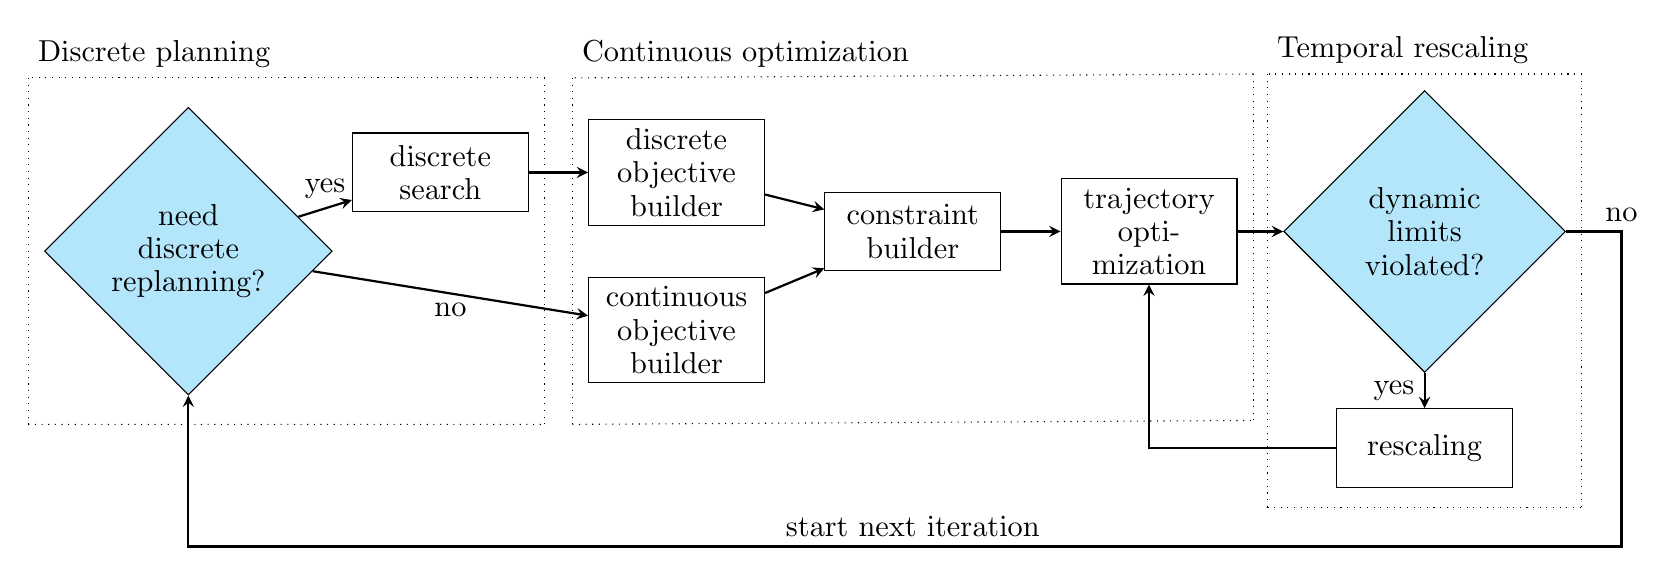
\begin{tikzpicture}[node distance = 2cm]
    \node (discrete) [decision, text width=2cm] {need discrete replanning?};
    \node (discretesearch) [process, right of=discrete, xshift=1.2cm, yshift = 1cm, text width = 2cm] {discrete search};
    \node (discobjbuild) [process, right of=discretesearch, xshift = 1cm, text width = 2cm] {discrete objective builder};
    \node (contobjbuild) [process, below of=discobjbuild, text width = 2cm] {continuous objective builder};
    \node (constraintbuild) [process, right of=discobjbuild, yshift = -0.75cm, xshift = 1cm, text width=2cm]
    {constraint builder};
    \node (trajopt) [process, right of=constraintbuild, xshift = 1cm, text width = 2cm] {trajectory optimization};
    \node (dynamiclimits) [decision, right of=trajopt, xshift = 1.5cm, text width = 2cm] {dynamic limits violated?};
    \node (rescale) [process, below of = dynamiclimits, text width = 2cm, yshift = -0.75cm] {rescaling};
    %\node (end) [io, right of = dynamiclimits, text width = 2cm, xshift = 2.5cm] {use trajectory for $\delta t$};
    
    \coordinate[above=2cm of discrete.west, xshift=-0.2cm, yshift=0.2cm] (c1);
    \coordinate[below=2cm of discrete.west, xshift=-0.2cm, yshift=-0.2cm] (c2);
    \coordinate[above=2cm of discretesearch.east, xshift = 0.2cm, yshift=-0.8cm] (c3);
    \coordinate[below=2cm of discretesearch.east, xshift = 0.2cm, yshift = -1.2cm] (c4);
    
    
    \coordinate[above=2cm of discobjbuild.west, xshift=-0.2cm, yshift=-0.8cm] (c5);
    \coordinate[below=2cm of discobjbuild.west, xshift=-0.2cm, yshift = -1.2cm] (c6);
    \coordinate[above=2cm of trajopt.east, xshift = 0.2cm] (c7);
    \coordinate[below=2cm of trajopt.east, xshift = 0.2cm, yshift=-0.4cm] (c8);
    
    
    \coordinate[above=2cm of dynamiclimits.west, xshift=-0.2cm] (c9);
    \coordinate[below=2cm of dynamiclimits.west, xshift=-0.2cm, yshift = -1.5cm] (c10);
    \coordinate[above=2cm of dynamiclimits.east, xshift = 0.2cm] (c11);
    \coordinate[below=2cm of dynamiclimits.east, xshift = 0.2cm, yshift = -1.5cm] (c12);
    
    \draw [arrow] (discrete) -- node[anchor=south] {yes} (discretesearch);
    \draw [arrow] (discrete) -- node[anchor=north] {no} (contobjbuild);
    \draw [arrow] (discretesearch) -- (discobjbuild);
    \draw [arrow] (discobjbuild) -- (constraintbuild);
    \draw [arrow] (contobjbuild) -- (constraintbuild);
    \draw [arrow] (constraintbuild) -- (trajopt);
    \draw [arrow] (trajopt) -- (dynamiclimits);
    \draw [arrow] (dynamiclimits) -- ++(2.5,0) node[anchor=south] {no} -- ++(0,-4) --  ++(-5,0) -- ++(-4,0) node[anchor=south] {start next iteration} -|   (discrete);
    \draw [arrow] (dynamiclimits) -- node[anchor=east] {yes} (rescale);
    \draw [arrow] (rescale) -| (trajopt);
    
    \node[right = 0cm of c1, yshift=0.3cm] {Discrete planning};
    \node[right = 0cm of c5, yshift=0.3cm] {Continuous optimization};
    \node[right = 0cm of c9, yshift=0.3cm] {Temporal rescaling};
    
    \draw [dotted] (c1) -- (c2);
    \draw [dotted] (c2) -- (c4);
    \draw [dotted] (c4) -- (c3);
    \draw [dotted] (c3) -- (c1);
    
    \draw [dotted] (c5) -- (c6);
    \draw [dotted] (c6) -- (c8);
    \draw [dotted] (c8) -- (c7);
    \draw [dotted] (c7) -- (c5);
    
    
    \draw [dotted] (c9) -- (c10);
    \draw [dotted] (c10) -- (c12);
    \draw [dotted] (c12) -- (c11);
    \draw [dotted] (c11) -- (c9);
\end{tikzpicture}
}
%\end{adjustbox}
\caption{Overview of the replanning pipeline.
}
\label{fig:flowchart}
\end{figure}

%\todo{DISCUSS: planning/execution overlap?}

\subsection{Discrete Planning} \label{discretePlanning}

In each planning iteration $K$ that corresponds to the current time $\psi$, we sense the neighbors' positions and compute the buffered voronoi cell $\cV_i(\psi)$.
We also assume that we have a current representation of the occupied space ($\cO(\psi)$), which can be achieved in practice by using LIDAR or RGB-D sensors.

We execute discrete planning if any of the following conditions is true:
\begin{enumerate}
    \item The original trajectory is not collision-free for the time horizon, i.e., $\exists t\in [\psi,\psi+\tau] : R_i(\vo_i(\psi)) \cap \cO(\psi) \neq \emptyset$,
    \item The first piece of the planned trajectory is outside robot $i$'s buffered voronoi cell, i.e., $\exists t\in [0, T^{K}_{i,1}] : \vf^{K}_{i,1}(t; T^{K}_{i,1}) \not\in \cV_i(\psi)$, or
    \item The planned trajectory is not collision-free for the time horizon, i.e., $\exists t\in [0,\tau] :  R_i(\vf^{K}_i(t)) \cap \cO(\psi) \neq \emptyset$.
\end{enumerate}
The first condition handles cases where previously unknown obstacles block the pre-planned path of a robot, the second case handles cases where previously unknown robots appear, and the third condition handles dynamic obstacles.

Discrete planning uses a dynamic receding horizon approach. First, we find the earliest time $\tau'\in [\min(\tau, T_i-\psi), T_i-\psi]$ where the original trajectory is collision-free with respect to both obstacles and other robots.
Second, we use a discrete graph search to find a path from the robots current location to $\vo_i(\psi+\tau')$ that avoids both static obstacles and other robots.
If $\tau'$ does not exist or no solution path exists, we skip the discrete planning stage.
Third, we use the first $l$ segments of the discrete path to uniformly place the new estimated control points on top of those segments.
In case the discrete path has fewer than $l$ segments, the last discrete segment is shared between multiple B\'ezier curves.
Finally, we adjust $T_{i,j}^K$ relative to the segment lengths and scale by $\tau'$, such that we would arrive at time $\psi+\tau'$ at location $\vo_i(\psi+\tau')$ if we would follow the discrete path using a uniform velocity.
However, to guarantee collision-free operation, we ensure that $T_{i,1}^K\geq \delta t$ in any case.

An example is shown in Fig.~\ref{fig:swap2:discrete}. 
Discrete planning is executed because the original trajectory (green dashed line) passes through an obstacle.
The earliest time to avoid the obstacle $\tau'$ is found such that the green robot re-joins its original trajectory after the obstacle.
A path that avoids both the static obstacle and the other (blue) robot is found (green dotted line) and has a total of six path segments.
The first four ($l=4$) segments are used to place new guesses of B\'ezier control points (blue, green, red, and cyan circles).
In this example, each curve has eight control points, although some of the points overlap.
The duration for each B\'ezier curve $T^{K}_{i,j}$ is adjusted according to the path length; for example, the duration of the segment with the red control points ($T_{i,3}^K$) is approximately twice as long as the duration of the segment with the green control points ($T_{i,2}^K$).





%\todo{need a statement that piece duration is at least delta t}

%\todo{when is ct introduced now?}

%WOLFGANG (text + pics)

\begin{figure}
\centering
\subfloat[Discrete path around an obstacle and other robot back to the original trajectory.]{
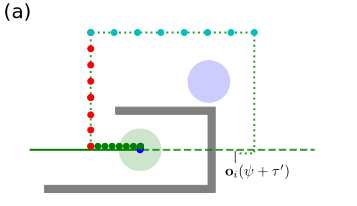
\includegraphics[width=0.45\textwidth]{images/swap2_discrete.pdf}
\label{fig:swap2:discrete}
}
\hfill
\subfloat[Continuous trajectory split into four pieces and respective hyperspaces.]{
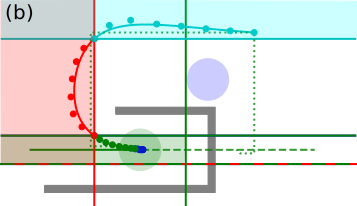
\includegraphics[width=0.45\textwidth]{images/swap2_cont_red.pdf}
\label{fig:swap2:cont}
}
% \begin{subfigure}[t]{0.48\textwidth}
% \centering
% 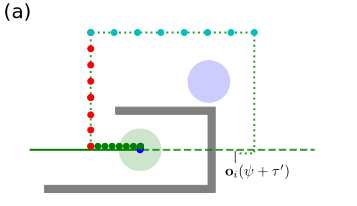
\includegraphics[width=1.0\textwidth]{images/swap2_discrete.pdf}
% \caption{Discrete path around an obstacle and other robot back to the original trajectory.}
% \label{fig:swap2:discrete}
% \end{subfigure} \hfill
% \begin{subfigure}[t]{0.48\textwidth}
% \centering
% 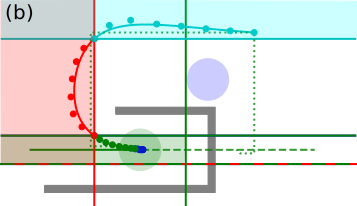
\includegraphics[width=1.0\textwidth]{images/swap2_cont_red.pdf}
% \caption{Continuous trajectory split into four pieces and respective hyperspaces.}
% \label{fig:swap2:cont}
% \end{subfigure}
\caption{
Snapshot at $t=3.9$.
}
\label{fig:swap2_2}
\end{figure}

% \begin{figure}
% \centering
% \subfloat[Voronoi decomposition.]{
% 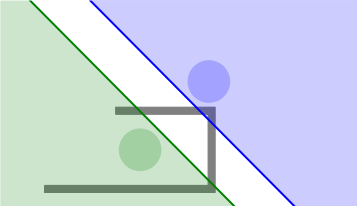
\includegraphics[width=0.48\textwidth]{images/swap2_voronoi.pdf}
% \label{fig:swap2:voronoi}
% }
% % \begin{subfigure}[b]{0.48\textwidth}
% % \centering
% % 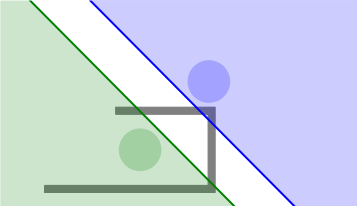
\includegraphics[width=1.0\textwidth]{images/swap2_voronoi.pdf}
% % \caption{Voronoi decomposition.}
% % \label{fig:swap2:voronoi}
% % \end{subfigure} \hfill
% % \begin{subfigure}[b]{0.45\textwidth}
% % \centering
% % 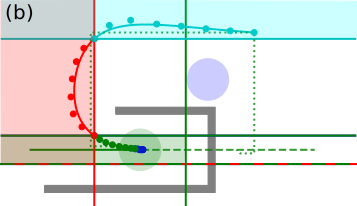
\includegraphics[scale=0.6]{images/swap2_cont_red.pdf}
% % \caption{Continuous trajectory split into four pieces and respective hyperspaces.}
% % \label{fig:swap2:cont}
% % \end{subfigure}
% \caption{
% %Snapshot at $t=3.9$.
% }
% \label{fig:swap2_3}
% \end{figure}

% consider moving ushape down (so green guy goes up)
% fig showing (one of the) initial conditions violated
% fig showing discrete plan and initial control points, color-coded by piece [might be just one figure]

\subsection{Continuous Optimization}\label{continuousOptimization}
In this stage, a quadratic optimization problem is solved where variables are the control points of the pieces concatenated together. If discrete planning is not performed, initial variables are copied from the previous iteration, and durations are set uniformly to $\frac{min(\tau,T_i-\psi)}{l}$. If discrete planning is performed, initial variables and durations are calculated from the discrete path as explained in Section~\ref{discretePlanning}. The objective $\cC$ that we minimize is defined as
\begin{align}
    \cC = \sum_{e=1}^{\cE} \lambda_e\int_{0}^{T^K_i} \left\|\frac{d^e\vf^{K}_i(t)}{dt^e}\right\|^2dt + \sum_{j=1}^{l} \theta_j \left\|\vP^{K}_{i,j,d} - \vchi_{j}\right\|^2 \label{costFunction}
\end{align}
where $\vchi_j$ is the point we want piece $j$ to end at. Refer to Section~\ref{bezierCurves} for the B\'ezier curve notation we use.

The first term of $\cC$ is the combination of integrated squared derivatives with weights $\lambda_e$ \cite{crazyplanning-ieeetro,richterISRR}. The second term of $\cC$ penalizes deviation from given end points for each piece of the trajectory with different weights $\theta_j$. In case discrete planning is performed, we require the end point of last piece to be in the final position of the discrete plan and do not constrain other pieces. If discrete planning is not performed, we require end points of each piece to get closer to the robot's position at corresponding times if it had followed the original trajectory, weighing each piece more than the previous one. This is an approximation we make for the cost function defined in Section~\ref{problemFormulation}. The construction of $H$ matrix defined in Section~\ref{trajectoryOptimization} for the first term is explained in \cite{crazyplanning-ieeetro}. The second term is a quadratic function of control points, hence it can be converted to an $H$ matrix and a $g$ vector as well.

For robot-to-robot collision avoidance, the buffered voronoi hyperplanes are computed according to equations \eqref{voronoiAlpha} and \eqref{voronoiBeta}. For each control point of the first piece, we add $m-1$ hyperspace constraints as
\begin{align}
    \alpha_i^j \cdot \vP^{K}_{i,1,\rho} \leq \beta_i^j, \rho \in \{0,1,...,d\}, j \in \{1,2,...,m\}\setminus\{i\}.
\end{align}

These constraints ensure that the first piece stays inside $\cV_i$ because of the convexity of $\cV_i$ and the convex hull property of B\'ezier curves. As long as $T^{i,K}_1 \geq \delta t$ and all other robots stay inside their voronoi cells up to time $\delta t$, we can be sure that no robot-to-robot collision will occur up to time $\delta t$. A sample buffered voronoi decomposition of the space is presented in Fig.~\ref{fig:swap2:voronoi}.

Remember at current global time $\psi$, $\cO(\psi)$ represents the occupied space. For each piece $j$, we calculate a set of SVM hyperplanes where hyperplane $M_j^b$ separates the initially guessed control points of the $j^{th}$ piece from the $b^{th}$ obstacle obtained from $\cO(\psi)$ using the method presented in Section~\ref{svmSection}. We shift these hyperplanes first towards to the obstacle than shift them back using the radius $r_i$ to account for the physical extend of the robot. We add hyperplane constraints as before requiring control points of the $j^{th}$ piece in the non-occupied side of each $M_j^b$ where $b\in \{1,2,...O\}$, $O$ being the number of non-occupied cells. These constraints ensure that no robot-to-obstacle constraint will occur up to time $\tau$. Fig.~\ref{fig:swap2:cont} shows the effective set of SVM hyperspaces for a $4$ piece trajectory.

After that we add continuity constraints that enforces continuity requirement between pieces.

Lastly, we add initial point constraints that enforce 
\begin{align*}
\frac{d^j\vf^{K}_i}{dt^j}(0) &= \frac{d^j\vp_i}{dt^j}\text{ for } j\in\{0,1,...,c\}\\
\end{align*}

All these constraints are linear as explained in Section~\ref{trajectoryOptimization}. Therefore, we indeed have a constructible quadratic optimization problem.

For an instance of a problem in dimension $n$ where the trajectory has $l$ pieces of degree $d$, number of variables in the optimization is $l(d+1)n$. Therefore the dimensins of the matrix $H$ is $l(d+1)n\times l(d+1)n$ and the vector $\vg$ is $l(d+1)\times 1$. If there are $m$ robots in the environment, buffered voronoi decomposition imposes $(m-1)(d+1)$ linear constraints. If there number of obstacles in the environment is $\uptheta$, SVM seperations impose $\uptheta l (d+1)$ linear constraints. If maximum required continuity is $c$, continuity requirements impose $(c+1)nl$ linear constraints. Therefore the matrix $A$ has $(m-1)(d+1) + \uptheta l(d+1) + (c+1)nl$ rows in total. For example, in 2-dimensional space with $4$ robots where the trajectory has $4$ pieces of degree $7$, the environment is occupied with $10$ obstacles and $C^{2}$ continuity is required, the number of variables would be $64$, and the number of linear constraints would be $368$.

% fig showing result from before (initial control points), hyperspaces (transparent, color-coded by piece), and resulting smooth trajectory (color-coded by piece).


\subsection{Temporal Rescaling} % might be part of overview
Since we use fixed durations for pieces and do not account for the dynamic limits of the robot during optimization, the resulting trajectory may violate dynamic limits of the robot. After trajectory optimization, we calculate the maximum magnitudes $\Gamma_j$ of $j^{th}$ derivatives of the curve, and check if for any $j$, $\Gamma_j > \gamma_j$, where $\gamma_j$ is the dynamic limit of the robot in $j^{th}$ derivation degree. If that is the case, we multiply durations $T^K_{i,j}$ of each piece by the same constant, and re-run the trajectory optimization with the same exact constraints using the previous result as the initial guess. If that is not the case, no temporal rescaling is needed and the trajectory is feasible.

% potentially more subsections about SVM, hyperplanes etc, as needed
% can look at T-RO paper for this part

\subsection{Theoretical Guarantees} %maybe
\begin{enumerate}
    \item As long as each robot $i$ follows the same rule, no robot-to-robot collision occurs. The maximum phase shift between robots is $\delta t$. If the dynamic limit $\gamma_1$ for velocities is uniform between robots, we can account for the phase shift by shifting each voronoi hyperplane $H_i^j$ by $\gamma_i \delta t$. Notice that this is a pessimistic shift, that does not take robot $j$'s extend into account. We can do even better if the geometry of the robots are uniform. This update gives \emph{no robot collision guarantee} even there is phase shift during the execution.
    \item The pessimistic shift mentioned above actually gives no robot-to-robot collision guarantee even if peers are non-cooperative that they do not obey buffered voronoi cell constraints.
    \item As long as obstacles are not moving, no robot-to-obstacle collision occurs. If we know the maximum velocity $\nu$ of the obstacles in the environment, we can avoid moving obstacles as well by shifting the SVM seperating hyperplanes by $\nu \delta t $. This update gives \emph{no obstacle collision guarantee} even the obstacles are moving.
\end{enumerate}
% see if we can formally get collision-free behavior (maybe only for synchronous execution) [see stanford paper]
% might be able to account for possible faceshift

\section{Evaluation}

We implement our approach in C++.
We use an occupancy grid as environment representation, because previous work has shown that such data structures can be updated in real-time on robots that are equipped with a LIDAR sensor or a RGB-D camera.
In particular, OctoMap~\cite{octomap} is an octree-based 3D occupancy grid that can be run on UAVs at at least \SI{4}{Hz} update rate~\cite{replanning-eth}.
OctoMaps are memory efficient, but update operations can show high execution time variance.
For local replanning, occupancy grids using ringbuffers as datastructures have been shown to achieve near constant execution time~\cite{replanning-usenko}.
Our implementation uses a simple pre-initialized 2D occupancy grid such that a physical robot implementation could leverage existing OctoMap or occupancy ringbuffer libraries easily.

We use the CVXGEN-package~\cite{cvxgen} to generate small QPs to find separating hyperplanes between controlpoints and obstacles.
As QP solvers we test with qpOASES~\cite{qpOASES} and OSQP~\cite{osqp}; both are open source and have been shown to work well in model predictive control scenarios. 

% TODO: figure out if there is some baseline (look at buffered vornoi paper)
% different use-case examples (see README.md)

\subsection{Simulation}
% scalability: #curves, #obstacles, #robots (voronoi constraint), qp-solver
% compare success rate with RVO2
%    describe typical examples (inline with the introduction)


% could talk about nlopt/ipopt "issues"; or: other subsection (e.g, other approaches)

\subsection{Physical Robots}


\section{Related Work}
\label{sec:relatedWork}

Our method is closely related to cooperative collision avoidance.
Such approaches assume that all robots follow the same strategy and can provide formal collision avoidance guarantees.
They typically find a subset of the configuration or control space that is safe to occupy for some time horizon.
A local planner can then optimize an arbitrary function as long as the robots stay in their respective safe configuration spaces.
Recent cooperative collision avoidance approaches include reciprocal velocity obstacles, buffered voronoi cells, and safety barrier certificates.
Methods based on reciprocal velocity obstacles (RVO)~\cite{RVO} assume that robots continue with constant velocity and compute the safe configuration space such that no other robot might collide for the time horizon. Many extensions of the RVO method have been proposed to support different kinds of robots, including heterogeneous teams, see \cite{epsilonCCA} for an extensive overview.
Buffered Voronoi Cells (BVC)~\cite{bufferedVoronoiCells} compute the safe configuration space for a robot by its Voronoi partition shifted by the physical extent of the robot. 
Safety barrier certificates achieves collision-free operation by modifying a user-specified controller such that no collision can occur~\cite{barrierCertificates}.
All approaches are decentralized and require only position (BVC and safety barrier certificates) or position and velocity estimates (RVO) of their neighbors.
Our robust motion execution approach uses cooperative collision avoidance at its core (specifically BVO), while extending it to minimize the difference to the original trajectories (rather than just a preferred velocity as in \cite{epsilonCCA}, preferred control input as in \cite{barrierCertificates}, or difference over a fixed time horizon as in \cite{bufferedVoronoiCells}).

Our realtime planning is inspired by our previous work on offline planning for robotic teams~\cite{crazyplanning-ieeetro}.
Here, a map of the environment, the specification of the robots, and the robots' start and goal locations are given.
The goal is to find smooth, collision-free trajectories that approximately minimize the total energy used.
The offline planner works in two stages: first, a discrete solution (on a discrete roadmap) is found using a graph search. Second, a quadratic program computes smooth trajectories for each robot, using the discrete result to define constraints and an initial solution.
Our robust motion execution uses the same optimization framework to generate trajectories, although with a different cost function.
We also use discrete search to quickly get out of local minima, but, unlike previous work, do so in a distributed manner.

While our approach naturally works in multi-robot settings, some of the methods are inspired by single-robot optimization and collision avoidance.
Using a discrete plan (generated by RRT*), polynomial trajectories can be generated using a quadratic program~\cite{richterISRR}.
In this case a unconstrained QP-formulation might be used, but obstacles cannot be directly taken into account.
Other basis functions, such as B-splines, allow us to add obstacles as linear hard constraints in a quadratic program~\cite{flores,tang}.
Local collision avoidance for single robots such as UAVs can be formulated as optimization problems~\cite{replanning-eth,replanning-usenko}.
In both cases collisions are considered as a soft constraint in the cost function using a Euclidean (Signed) Distance Field.
In contrast, our formulation uses a hard constraint and therefore guarantees collision-free execution (or easy error-case detection in case our quadratic program is infeasible).
The optimization can use a discrete plan as initial guess~\cite{replanning-eth} or shift the existing trajectory based on newly appearing obstacles~\cite{replanning-usenko}.
In contrast, our approach shifts the existing trajectory whenever possible, while falling back to an efficient discrete planner with dynamic receding horizon to avoid local minima.

% multi-robot:
% BVC, RVO, barrier certificate

% stanford paper


% tu munich paper
%\cite{replanning-usenko}

% t-ro paper (& other traj opt papers)
%\cite{crazyplanning-ieeetro}
%\cite{tang}
%\cite{flores}

% other traj opt:
%\cite{replanning-eth}
%\cite{richterISRR}


\section{Conclusion}

%
% ---- Bibliography ----
%
\bibliographystyle{spmpsci}
\bibliography{bibliography}

\section{TODO}

\todo{why are functions marked as vectors?}

% Monday - Thursday/ Saturday: writing
% 
% May 11/13: physical robot experiments [warehouse]
% May 14: paper ready for review within the lab
% Tuesday May 22: submission

\end{document}
